% Options for packages loaded elsewhere
\PassOptionsToPackage{unicode}{hyperref}
\PassOptionsToPackage{hyphens}{url}
\PassOptionsToPackage{dvipsnames,svgnames,x11names}{xcolor}
%
\documentclass[
  12pt,
]{article}
\usepackage{amsmath,amssymb}
\usepackage{lmodern}
\usepackage{iftex}
\ifPDFTeX
  \usepackage[T1]{fontenc}
  \usepackage[utf8]{inputenc}
  \usepackage{textcomp} % provide euro and other symbols
\else % if luatex or xetex
  \usepackage{unicode-math}
  \defaultfontfeatures{Scale=MatchLowercase}
  \defaultfontfeatures[\rmfamily]{Ligatures=TeX,Scale=1}
\fi
% Use upquote if available, for straight quotes in verbatim environments
\IfFileExists{upquote.sty}{\usepackage{upquote}}{}
\IfFileExists{microtype.sty}{% use microtype if available
  \usepackage[]{microtype}
  \UseMicrotypeSet[protrusion]{basicmath} % disable protrusion for tt fonts
}{}
\makeatletter
\@ifundefined{KOMAClassName}{% if non-KOMA class
  \IfFileExists{parskip.sty}{%
    \usepackage{parskip}
  }{% else
    \setlength{\parindent}{0pt}
    \setlength{\parskip}{6pt plus 2pt minus 1pt}}
}{% if KOMA class
  \KOMAoptions{parskip=half}}
\makeatother
\usepackage{xcolor}
\usepackage[margin=1in]{geometry}
\usepackage{color}
\usepackage{fancyvrb}
\newcommand{\VerbBar}{|}
\newcommand{\VERB}{\Verb[commandchars=\\\{\}]}
\DefineVerbatimEnvironment{Highlighting}{Verbatim}{commandchars=\\\{\}}
% Add ',fontsize=\small' for more characters per line
\usepackage{framed}
\definecolor{shadecolor}{RGB}{248,248,248}
\newenvironment{Shaded}{\begin{snugshade}}{\end{snugshade}}
\newcommand{\AlertTok}[1]{\textcolor[rgb]{0.94,0.16,0.16}{#1}}
\newcommand{\AnnotationTok}[1]{\textcolor[rgb]{0.56,0.35,0.01}{\textbf{\textit{#1}}}}
\newcommand{\AttributeTok}[1]{\textcolor[rgb]{0.77,0.63,0.00}{#1}}
\newcommand{\BaseNTok}[1]{\textcolor[rgb]{0.00,0.00,0.81}{#1}}
\newcommand{\BuiltInTok}[1]{#1}
\newcommand{\CharTok}[1]{\textcolor[rgb]{0.31,0.60,0.02}{#1}}
\newcommand{\CommentTok}[1]{\textcolor[rgb]{0.56,0.35,0.01}{\textit{#1}}}
\newcommand{\CommentVarTok}[1]{\textcolor[rgb]{0.56,0.35,0.01}{\textbf{\textit{#1}}}}
\newcommand{\ConstantTok}[1]{\textcolor[rgb]{0.00,0.00,0.00}{#1}}
\newcommand{\ControlFlowTok}[1]{\textcolor[rgb]{0.13,0.29,0.53}{\textbf{#1}}}
\newcommand{\DataTypeTok}[1]{\textcolor[rgb]{0.13,0.29,0.53}{#1}}
\newcommand{\DecValTok}[1]{\textcolor[rgb]{0.00,0.00,0.81}{#1}}
\newcommand{\DocumentationTok}[1]{\textcolor[rgb]{0.56,0.35,0.01}{\textbf{\textit{#1}}}}
\newcommand{\ErrorTok}[1]{\textcolor[rgb]{0.64,0.00,0.00}{\textbf{#1}}}
\newcommand{\ExtensionTok}[1]{#1}
\newcommand{\FloatTok}[1]{\textcolor[rgb]{0.00,0.00,0.81}{#1}}
\newcommand{\FunctionTok}[1]{\textcolor[rgb]{0.00,0.00,0.00}{#1}}
\newcommand{\ImportTok}[1]{#1}
\newcommand{\InformationTok}[1]{\textcolor[rgb]{0.56,0.35,0.01}{\textbf{\textit{#1}}}}
\newcommand{\KeywordTok}[1]{\textcolor[rgb]{0.13,0.29,0.53}{\textbf{#1}}}
\newcommand{\NormalTok}[1]{#1}
\newcommand{\OperatorTok}[1]{\textcolor[rgb]{0.81,0.36,0.00}{\textbf{#1}}}
\newcommand{\OtherTok}[1]{\textcolor[rgb]{0.56,0.35,0.01}{#1}}
\newcommand{\PreprocessorTok}[1]{\textcolor[rgb]{0.56,0.35,0.01}{\textit{#1}}}
\newcommand{\RegionMarkerTok}[1]{#1}
\newcommand{\SpecialCharTok}[1]{\textcolor[rgb]{0.00,0.00,0.00}{#1}}
\newcommand{\SpecialStringTok}[1]{\textcolor[rgb]{0.31,0.60,0.02}{#1}}
\newcommand{\StringTok}[1]{\textcolor[rgb]{0.31,0.60,0.02}{#1}}
\newcommand{\VariableTok}[1]{\textcolor[rgb]{0.00,0.00,0.00}{#1}}
\newcommand{\VerbatimStringTok}[1]{\textcolor[rgb]{0.31,0.60,0.02}{#1}}
\newcommand{\WarningTok}[1]{\textcolor[rgb]{0.56,0.35,0.01}{\textbf{\textit{#1}}}}
\usepackage{longtable,booktabs,array}
\usepackage{calc} % for calculating minipage widths
% Correct order of tables after \paragraph or \subparagraph
\usepackage{etoolbox}
\makeatletter
\patchcmd\longtable{\par}{\if@noskipsec\mbox{}\fi\par}{}{}
\makeatother
% Allow footnotes in longtable head/foot
\IfFileExists{footnotehyper.sty}{\usepackage{footnotehyper}}{\usepackage{footnote}}
\makesavenoteenv{longtable}
\usepackage{graphicx}
\makeatletter
\def\maxwidth{\ifdim\Gin@nat@width>\linewidth\linewidth\else\Gin@nat@width\fi}
\def\maxheight{\ifdim\Gin@nat@height>\textheight\textheight\else\Gin@nat@height\fi}
\makeatother
% Scale images if necessary, so that they will not overflow the page
% margins by default, and it is still possible to overwrite the defaults
% using explicit options in \includegraphics[width, height, ...]{}
\setkeys{Gin}{width=\maxwidth,height=\maxheight,keepaspectratio}
% Set default figure placement to htbp
\makeatletter
\def\fps@figure{htbp}
\makeatother
\setlength{\emergencystretch}{3em} % prevent overfull lines
\providecommand{\tightlist}{%
  \setlength{\itemsep}{0pt}\setlength{\parskip}{0pt}}
\setcounter{secnumdepth}{5}
\newlength{\cslhangindent}
\setlength{\cslhangindent}{1.5em}
\newlength{\csllabelwidth}
\setlength{\csllabelwidth}{3em}
\newlength{\cslentryspacingunit} % times entry-spacing
\setlength{\cslentryspacingunit}{\parskip}
\newenvironment{CSLReferences}[2] % #1 hanging-ident, #2 entry spacing
 {% don't indent paragraphs
  \setlength{\parindent}{0pt}
  % turn on hanging indent if param 1 is 1
  \ifodd #1
  \let\oldpar\par
  \def\par{\hangindent=\cslhangindent\oldpar}
  \fi
  % set entry spacing
  \setlength{\parskip}{#2\cslentryspacingunit}
 }%
 {}
\usepackage{calc}
\newcommand{\CSLBlock}[1]{#1\hfill\break}
\newcommand{\CSLLeftMargin}[1]{\parbox[t]{\csllabelwidth}{#1}}
\newcommand{\CSLRightInline}[1]{\parbox[t]{\linewidth - \csllabelwidth}{#1}\break}
\newcommand{\CSLIndent}[1]{\hspace{\cslhangindent}#1}
\usepackage{polyglossia}
\setmainlanguage{turkish}
\usepackage{booktabs}
\usepackage{caption}
\captionsetup[table]{skip=10pt}
\ifLuaTeX
  \usepackage{selnolig}  % disable illegal ligatures
\fi
\IfFileExists{bookmark.sty}{\usepackage{bookmark}}{\usepackage{hyperref}}
\IfFileExists{xurl.sty}{\usepackage{xurl}}{} % add URL line breaks if available
\urlstyle{same} % disable monospaced font for URLs
\hypersetup{
  pdftitle={Yıllık Gelirdeki Farklılıklara Sebep Olan Faktörler},
  pdfauthor={Başak Aydın},
  colorlinks=true,
  linkcolor={Maroon},
  filecolor={Maroon},
  citecolor={Blue},
  urlcolor={blue},
  pdfcreator={LaTeX via pandoc}}

\title{Yıllık Gelirdeki Farklılıklara Sebep Olan Faktörler}
\author{Başak Aydın\footnote{Öğrenci Numarası, \href{https://github.com/basakaaydin/istatistikfinal}{Github Repo}}}
\date{}

\begin{document}
\maketitle
\begin{abstract}
Yıllık geliri etkileyen ve değişikliklere sebep olan birçok faktör bulunmaktadır.Bunlar;cinsiyet,ırk,yaş,eğitim durumu gibi faktörlerdir.Bu çalışmada UCI Machine Learning Repositery üzerinden alınan veri seti ile yıllık gelir üzerinde farklılıklara sebep olan faktörlerin analiz edilerek ve yorumlanarak incelenmesidir.
\end{abstract}

\hypertarget{giriux15f}{%
\section{Giriş}\label{giriux15f}}

Yapmış olduğum bu çalışmada araştırma sorum yıllık gelirdeki değişimleri etkileyen faktörler nelerdir sorusuna dayanmaktadır.Bu sorudan yola çıkarak elde ettiğim sonuçların gelir üzerindeki etkisini incelemek ve veriyi analiz etmek projemin konusunu oluşturmaktadır.Araştırmama dair kullandığım veri setini UCI Machine Learning Repository sitesi üzerinden aldım.Bu veri seti nüfus sayımı verilerine dayanarak yıllık gelirin 50.000\$'ı aşıp aşmadığını incelemektedir.Veri setim toplam 14 değişken ve 48.842 gözlem içermektedir.Değişkenler age,workclass,fnlwgt,education,education-num,marital-status,occupation,relationship,race,sex,capital gain,capital loss,hours per week,native country'den oluşmaktadır.

\hypertarget{uxe7alux131ux15fmanux131n-amacux131}{%
\subsection{Çalışmanın Amacı}\label{uxe7alux131ux15fmanux131n-amacux131}}

Bu araştırmada yaş,etnik grup,cinsiyet,eğitim,medeni hali gibi değişkenlerine göre gelirin farklılık gösterip göstermediği incelenmiştir.

Birçok ülke,kurum ve kuruluşlar iş dünyasında ayrım yapmaksızın fırsat eşitliğine yönelik çeşitli hükümlerde bulunsa da iş hayatında dolayısıyla ücretlerde çok bariz farklılıklar bulunmaktadır.

Bu farklılıkların hangi değişkenlerden kaynaklandığını tespit ederek,yorumlayıp,bir bakış açısı oluşturup,çözümler sunabilmek bu çalışmanın amacıdır.

\hypertarget{literatuxfcr}{%
\subsection{Literatür}\label{literatuxfcr}}

İş gücü piyasasında cinsiyet,etnik köken,ırk,yaş,din gibi birçok faktörlerden kaynaklanan ayrımcılığın ABD,Çin,Güney Kore ve bunun gibi birçok güçlü devletlerde bariz bir sorun olduğunu görüyoruz.Ayrımcılık özellikle iş ortamında ücret,iş alma ve terfi konularında yoğunlaşıyor.Bu tarz ayrımcılıklar işgücü piyasalarının gelişimini ve işleyişini aynı zamanda geliri etkileyen en temel sorunlardan birisidir.Kişisel ücret farklılıklarında aynı birimde çalışan işçilerin yaş ve cinsiyetine göre çok büyük faklılıkların olduğu bariz.Eşit işe eşit ücret sağlanması gerektiği halde bu göz ardı ediliyor.Bunun en iyi örneği kadın işçiye aynı işi yapması için erkek işçiden daha az ücret ödenmesi durumudur.Toplumsal cinsiyet eşitsizliği ya da bir başka deyişle cinsiyete dayalı işbölümü temelinde kadınlar erkekler ile aynı eğitim düzeyine ve mesleki kıdeme sahip olsalar bile sadece kadın olmalarından kaynaklı cinsiyetçi ücret ayrımına maruz kalmaktadır.Bunu yıllık gelire vurduğumuzda kadınlardaki yıllık gelir erkeklerdekine göre daha düşük bir meblağ olarak istatistiklere yansıyor. @seher2016icsgucu

İş gücü piyasasında cinsiyet dışında medeni durum,yaş,eğitim düzeyi,mesleki tecrübe ve verimlilik gibi iş gücünün özelliğinden kaynaklanan ücret/gelir farklılıkları da bulunmaktadır.Sektör özellikleri ve bölgeler arası ücret farklılıklarından kaynaklanan yıllık gelir farklılıkları da bulunmaktadır.İşgücü piyasalarında işleri ve ücretleri farklılaştıran bir başka unsur da firma ölçeğidir. Hemen her yerde ve zamanda gözlenen bir durum büyük firmalarda ücretlerin küçük firmalara oranla daha yüksek olmasıdır. Büyük firmalarda ücretlerin yüksek olması işleri birbirinden heterojen kılarak ücretlerin farklılaşmasına yol açar. @maktav2019icsgucu

Etkin Ücret Teorisine göre işçiyi denetlemenin ve performansını ölçmenin zor olduğu, işçinin hatalı üretim yapmasının maliyetli olduğu, işin belirli bir süre spesifik işyerinde eğitim gerektirdiği durumlarda işverenlerin istekli olarak piyasa denge ücretinin üstünde ücret (etkin ücret ödemesi) verdikleri söylenebilir. Etkin ücret ödemelerinin işleri birbirinden farklı (heterojen) hale getirerek emek piyasalarında ücret farklılıklarına neden olabileceğini belirtmek gerekir. Benzeri özelliklere sahip iki işçiden birisi etkin ücret uygulamasının yapıldığı firma veya işkolunda çalışıyorsa diğerinden daha yüksek ücret alabilmektedir. @blackaby1991industry
Bir diğer gelirdeki farklılıkların nedeni ise ırktır.Siyah ve beyaz ayrımı geçmişten bugüne devam eden bir sorundur.Siyah erkeklerin hala birçok işyerinde aynı meslekte çalışan beyaz erkeklerden daha düşük bir ücret aldığını istatistikler birçok kez göstermiştir.Bunun yanı sıra gelirdeki farklılıklar ırksal eğitim eşitsizliği ile de doğru orantılı.Örneğin ABD'deki istatistiklere göre beyaz ailelerin \%39'u lisans eğitimi veya yüksek eğitim mezunu iken siyahi ve hispanik ailelerde bu oran \%23 ve \%17'dir.Irklar arasındaki eğitim durumu farkı iş hayatında daha az ücretle çalışma ya da tercih edilmeme gibi durumlara yol açıyor. @stolzenberg1975education

Sonuç olarak iş gücü piyasasında karşılaştığımız birçok değişken faktör gelirdeki farklılıkların neyden,hangi değişkenlerden kaynaklandığını anlamamıza ve analiz etmemize yardımcı olmaktadır.

\hypertarget{veri}{%
\section{Veri}\label{veri}}

Veri setimi Ucı machine learning repositoryden alarak excel dosyasına aktardım.Bazı NA gözlemler vardı onları düzenledim ve csv dosyasına dönüştürerek analizime dahil ettim.

Analize ait R kodları bu bölümde başlamalıdır. Bu bölümde veri setini R'a aktaran ve özet istatistikleri üreten kodlar yer almalıdır.

Rmd dosyasında kod bloklarının bazılarında kod seçeneklerinin düzenlendiğine dikkat edin.

\texttt{echo=FALSE} seçeneği ile kodların türetilen pdf dosyasında görünmesini engelleyin ve sonuçlarınızı tablo halinde rapor edin.

\begin{table}[ht]
\centering
\caption{Özet İstatistikler} 
\label{tab:ozet}
\begin{tabular}{lccccc}
  \toprule
 & Ortalama & Std.Sap & Min & Medyan & Mak \\ 
  \midrule
capital gain & 7663.83 & 422.97 & 1055.00 & 7688.00 & 15024.00 \\ 
  hours per week & 40.44 & 12.35 & 1.00 & 40.00 & 99.00 \\ 
  yearly income & 43024.94 & 700.03 & 37000.00 & 43000.00 & 70000.00 \\ 
   \bottomrule
\end{tabular}
\end{table}

\hypertarget{yuxf6ntem-ve-veri-analizi}{%
\section{Yöntem ve Veri Analizi}\label{yuxf6ntem-ve-veri-analizi}}

Bu bölümde veri setindeki bilgileri kullanarak çalışmanın amacına ulaşmak için kullanılacak yöntemleri açıklayın. Derste işlenen/işlenecek olan analiz yöntemlerinden (Hipotez testleri ve korelasyon analizi gibi) çalışmanın amacına ve veri setine uygun olanlar bu bölümde kullanılmalıdır. {[}@newbold:2003; @ozsoy:2010; @ozsoy:2014{]}

Örneğin, regresyon analizi gerçekleştiriyorsanız tahmin ettiğiniz denklemi bu bölümde tartışınız. Denklemlerinizi ve matematiksel ifadeleri \(LaTeX\) kullanarak yazınız.

\[
Y_t = \beta_0 + \beta_N N_t + \beta_P P_t + \beta_I I_t + \varepsilon_t
\]

Bu bölümde analize ilişkin farklı tablolar ve grafiklere yer verilmelidir. Çalışmanıza uygun biçimde histogram, nokta grafiği (Şekil \ref{fig:plot} gibi), kutu grafiği, vb. grafikleri bu bölüme ekleyiniz. Şekillerinize de gerekli göndermeleri bir önceki cümlede gösterildiği gibi yapınız.

\begin{Shaded}
\begin{Highlighting}[]
\NormalTok{veri }\SpecialCharTok{\%\textgreater{}\%} 
\FunctionTok{ggplot}\NormalTok{(}\FunctionTok{aes}\NormalTok{(}\AttributeTok{x =}\NormalTok{ Age, }\AttributeTok{y =} \StringTok{\textasciigrave{}}\AttributeTok{yearly income}\StringTok{\textasciigrave{}}\NormalTok{)) }\SpecialCharTok{+}
  \FunctionTok{geom\_point}\NormalTok{() }\SpecialCharTok{+}
  \FunctionTok{geom\_smooth}\NormalTok{() }\SpecialCharTok{+}
  \FunctionTok{scale\_x\_continuous}\NormalTok{(}\StringTok{"age"}\NormalTok{) }\SpecialCharTok{+} 
  \FunctionTok{scale\_y\_continuous}\NormalTok{(}\StringTok{"yearly income"}\NormalTok{)}
\end{Highlighting}
\end{Shaded}

\begin{figure}

{\centering 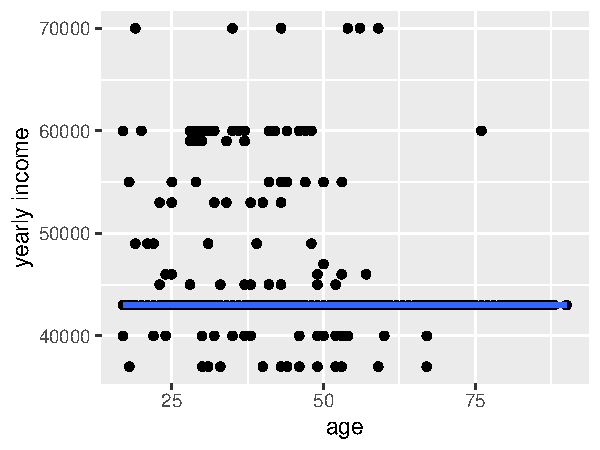
\includegraphics{final-ödev_files/figure-latex/plot-1} 

}

\caption{Muhteşem Bir Grafik}\label{fig:plot}
\end{figure}

\hypertarget{sonuuxe7}{%
\section{Sonuç}\label{sonuuxe7}}

Bu bölümde çalışmanızın sonuçlarını özetleyiniz. Sonuçlarınızın başlangıçta belirlediğiniz araştırma sorusuna ne derece cevap verdiğini ve ileride bu çalışmanın nasıl geliştirilebileceğini tartışınız.

\textbf{Kaynakça bölümü Rmarkdown tarafından otomatik olarak oluşturulmaktadır. Taslak dosyada Kaynakça kısmında herhangi bir değişikliğe gerek yoktur.}

\textbf{\emph{Taslakta bu cümleden sonra yer alan hiçbir şey silinmemelidir.}}

\newpage

\hypertarget{references}{%
\section{Kaynakça}\label{references}}

\hypertarget{refs}{}
\begin{CSLReferences}{0}{0}
\end{CSLReferences}

\end{document}
